\documentclass[a4paper]{article}
\usepackage{amsmath}
\usepackage{amsfonts}
\usepackage{amsthm}
\usepackage{amssymb}
\usepackage[english]{babel}
\usepackage{float}
\usepackage{graphicx}
\usepackage{hyperref}
\usepackage[utf8]{inputenc}
\usepackage{listings}
\usepackage{xcolor}
%% \usepackage{subfigure}
\usepackage{graphicx}
\usepackage{subcaption}
\usepackage{stmaryrd}

\usepackage{a4wide}
\usepackage{url}

\usepackage{appendix}

\graphicspath{{imgs/}} %Setting the graphicspath

\lstset{
  frame=tb,
  language=Python,
  aboveskip=3mm,
  belowskip=3mm,
  showstringspaces=false,
  formfeed=newpage,
  tabsize=4,
  comment=[l]{\#},
  breaklines=true,
  morekeywords={models, lambda, forms}
}

\newcommand{\prob}[1]{\mathbb{P}\left(#1\right)}
\newcommand{\expect}[1]{\mathbb{E}\left(#1\right)}
\newcommand{\bt}[1]{\mathbf{#1}}
\newcommand{\avg}[1]{\sum_{i=1}^{#1}X_i}
\newcommand*{\QEDA}{\hfill\ensuremath{\blacksquare}}%

\newcommand{\nt}{\text}
\newcommand{\lagr}{\mathcal{L}}
\newcommand{\isum}{\sum^\infty_}
\newcommand{\f}{$f$}

\title{\vspace{-5cm} Numerical Optimization \\ Re-exam Handin 3}
\author{Dmitry Serykh (qwl888)}

\begin{document}
\maketitle
\section{The Setup}
I implemented the stepest descent and Newton's algorithms using the
backtracking line search in order to find the step length (Algorithm 3.1).

\subsection{Hessian Modification for the Newton's Method}
The problem with Newton's method is that for non-convex functions, the Newton's step\\
$p_k^{N} = -\nabla^2 f(x_k)^{-1} \nabla f(x_k)$ may not be in a descent direction and Hessian could
be non-invertible. I have modified the Hessian using the Cholesky with Added
Multiple of Identity method (Algorithm 3.3). A value of $\tau I$ is added to the
Hessian. If the Cholesky factorization of the resulting matrix succeeds, we are done.
Otherwise, a new value of $\tau$ is calculated.

\subsection{Parameters}
After some testing, I have determined that for my implementation, different
parameters must be used for the steepest descent and Newton's methods.
Following parameter values were used:

\begin{itemize}
\item \textbf{Initial step length.} For the Netwon's method, I have used the natural
  value of ($\bar{\alpha}=1$). For the stepest descent, I empirically found the value
  of $\bar{\alpha} = 0.1$  to perform best
\item \textbf{Factor $\rho$}. For the stepest descent, I used the value of
  $\rho = 0.2$. For the Newton's method, I have used the value of $\rho=0.5$.
\item \textbf{Constant $c$}. For both methods, I have used to value of $c=10^{-5}$.
\item \textbf{Stopping criteria}. For both methods, I have used
  $\varepsilon = \| \nabla f\| = 10^{-7}$. Furthermore, I have terminated the
  algorithm at 20000 iterations. However this was only relevant to the steepest descent.
\item \textbf{Value of $\beta$}. For the Hessian Modification (Algorithm 3.3), I
  have used a value of $\beta=10^{-3}$.
\end{itemize}



\section{Testing protocol}
In order to test the effectiveness of my implementation, I came up with a
testing protocol, where I used following metrics:

\begin{itemize}
\item The convergence plots with the number of iteration on the x-scale and the
  log of the Euclidean distance between the current value of $x$ and the
  optimum. The results can be seen on Figure \ref{plt1}. I applied the low shelf
  to the results, so anything would stop at $10^{-6}$.
\item The convergence plots with the gradient magnitude.
  The results can be seen on Figure \ref{plt2}. 
\item \textbf{Efficiency}. The number of steps until the gradient magnitude reaches $10^{-7}$. The
  results can be seen on Table \ref{table2}.
\item \textbf{Accuracy}. The Euclidean distance to the optimum at the
  termination point. The results can be seen on Table \ref{table1}.
\end{itemize}
I used a random starting point taken from the uniform distribution in the
interval between $-10$ to $10$ and repeated each optimization 100 times for both
metrics and took the average. This was done to remove the influence of the
starting position from the results of the optimization. I used the mean 
to minimize the effect of the outliers,
which is important due to the stochastic nature of the algorithm. 
\begin{table}[]
\centering
\begin{tabular}{|l|l|l|l|l|l|}
\hline
                 & $f_1$         & $f_2$         & $f_3$       & $f_4$       & $f_5$       \\ \hline
stepest descent & $1.437\cdot10^{-4}$ & $7.59\cdot10^{-4}$ & $1.44\cdot10^{-10}$ & $6.51\cdot10^{-7}$ & $1.13\cdot 10^{-4}$ \\ \hline
newton           & $0.0$      & $8.15\cdot10^{-8}$ & $4.59\cdot10^{-16}$ & $6.4\cdot10^{-7}$  & $4.56\cdot10^{-7}$ \\ \hline
\end{tabular}
\caption{Average value of distance to the optimum at algorithm termination for 100 random starting points in the interval $[-10,10]$}
\label{table1}
\end{table}

\begin{table}[]
\centering
\begin{tabular}{|l|l|l|l|l|l|}
\hline
                 & $f_1$ & $f_2$   & $f_3$  & $f_4$  & $f_5$ \\ \hline
stepest descent & $3392$ & $6991$ & $5546$ & $488$ & $52$ \\ \hline
newton           & $1$  & $30$   & $16$  & $29$  & $2 $ \\ \hline
\end{tabular}
\caption{Average number of iterations until algorithm termination for 100 random starting points in the interval $[-10,10]$}
\label{table2}
\end{table}

\begin{figure}[]
    \centering
    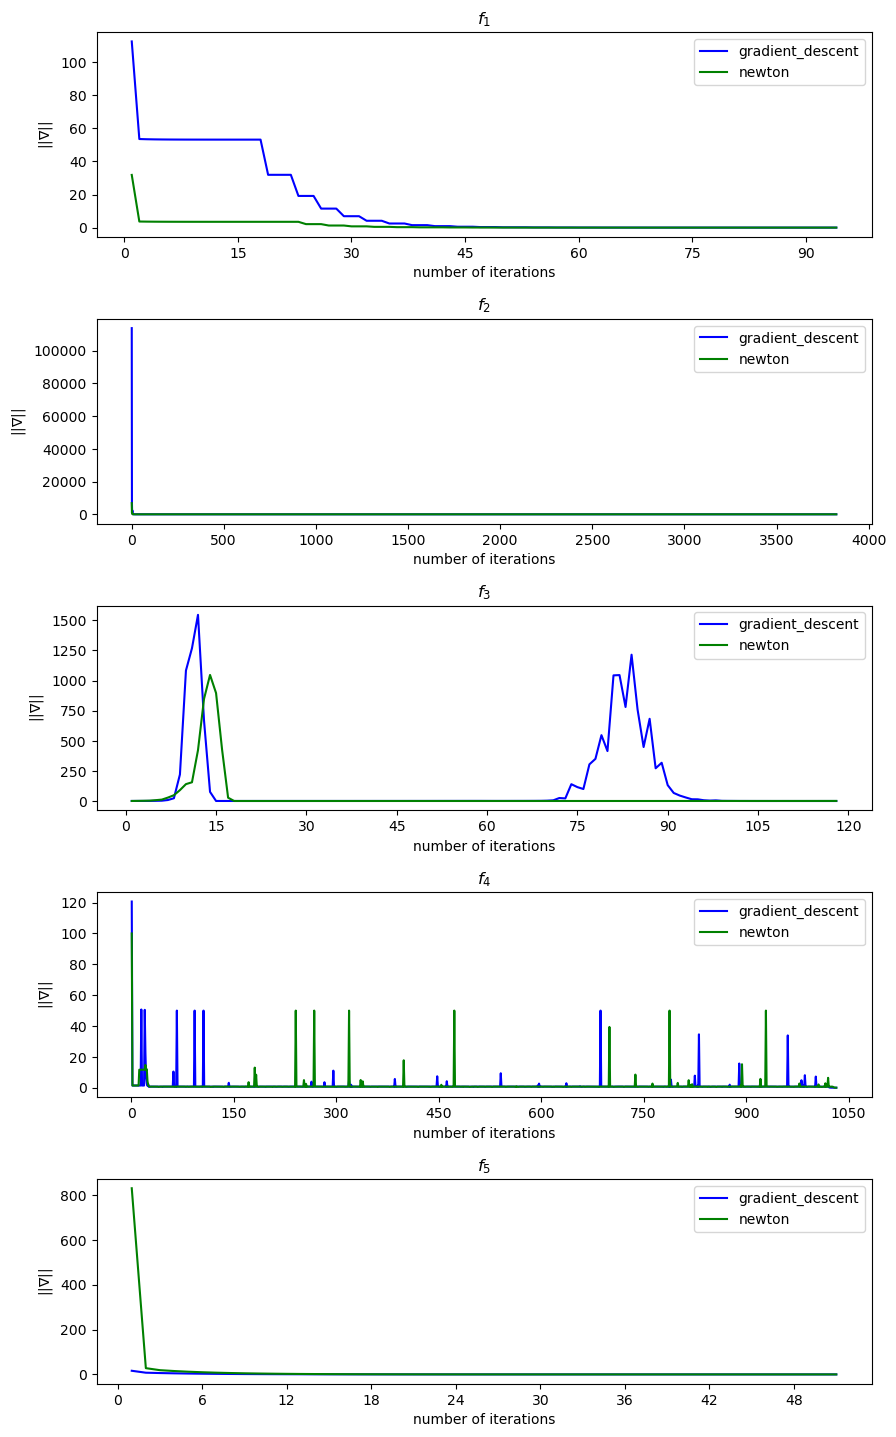
\includegraphics[width=0.6\textwidth]{plt_grad100.png}
    \caption{Convergence plot with norm of the gradient on y-axis}
  \label{plt1}
\end{figure}

\begin{figure}[]
    \centering
    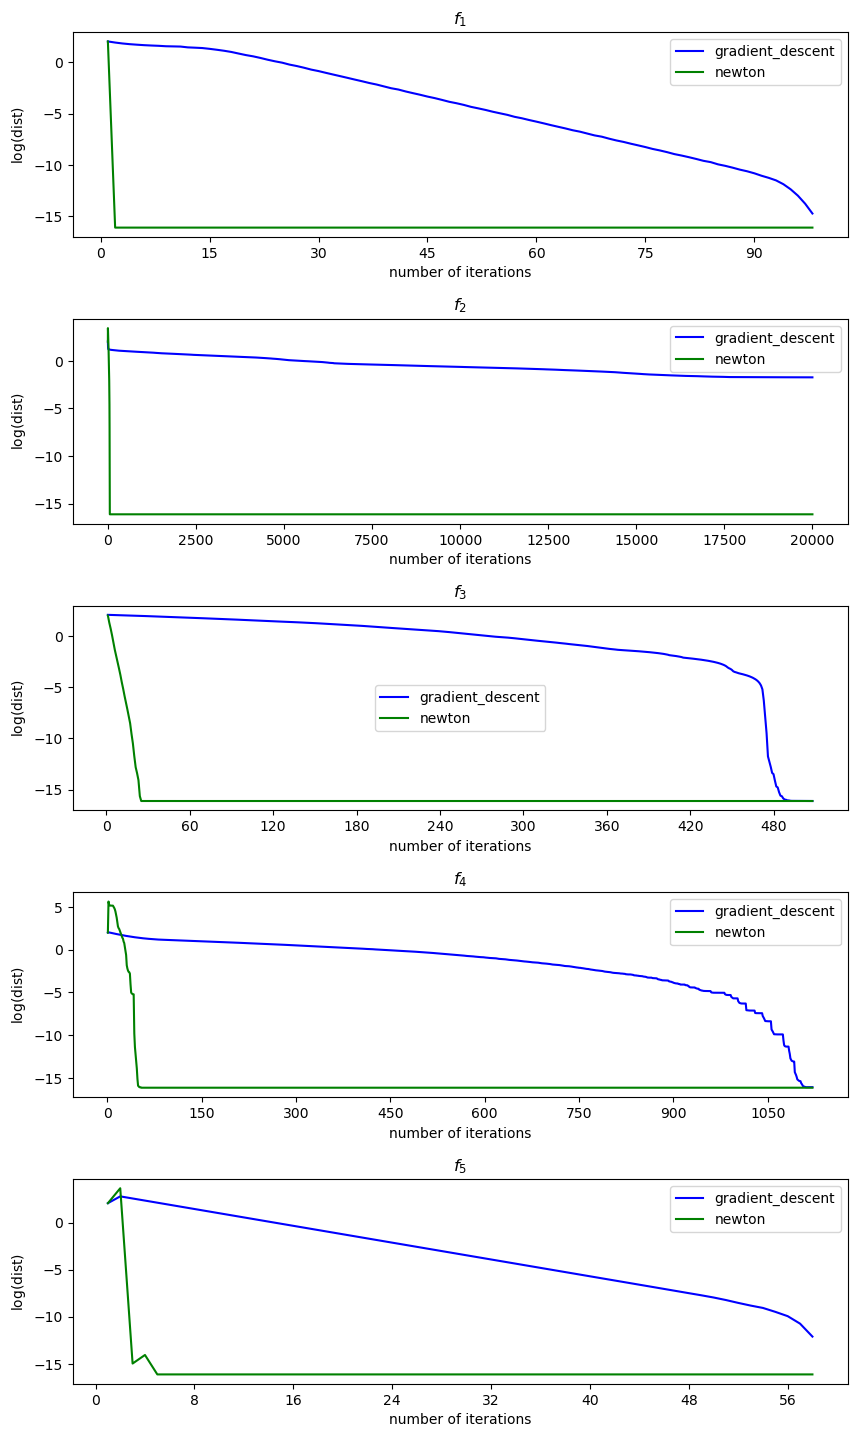
\includegraphics[width=0.8\textwidth]{plt_dist100.png}
    \caption{Convergence plot with log of euclidean distance on the y-axis}
  \label{plt2}
\end{figure}

\section{Theoretical Part}
\subsection{Exercise 3.7}
Let us start by looking at the expression:
\[
\begin{aligned}
\nabla f(x_k) &= Q\left(x_{k}-x^{*}\right)\\
Q^{-1}\nabla f(x_k) &= \left(x_{k}-x^{*}\right)
\end{aligned}
\]
$f(x_k)^T = \left(x_{k}-x^{*}\right)^TQ^T = \left(x_{k}-x^{*}\right)^TQ$, since $Q$ is symmetric, then:
\[
\begin{aligned}
\nabla f(x_k)^T Q^{-1}\nabla f(x_k) &= \left(x_{k}-x^{*}\right)^TQ\left(x_{k}-x^{*}\right)\\
 \| x_{k} - x^* \|_Q^2 &= \nabla f(x_k)^T Q^{-1}\nabla f(x_k)
\end{aligned}
\]
This would be useful later.\\\\
By the definition of the step direction in the Steepest Descent method, and subtracting the $x^*$ on
both sides, we have:
\[
x_{k+1} - x^* = x_k - x^* - \alpha\nabla f(x_k)
\]
Then, by the definition of the Q-weighted norm, we have:
\[
\begin{aligned}
  \left\|x_{k+1}-x^{*}\right\|_{Q}^{2} &=\left(x_{k}-x^{*}-\alpha \nabla f(x_k)\right)^{T} Q\left(x_{k}-x^{*}-\alpha
  \nabla f(x_k)\right) \\
  &=\left(x_{k}-x^{*}\right)^{T} Q\left(x_{k}-x^{*}\right)-2 \alpha \nabla f(x_k)^{T}
  Q\left(x_{k}-x^{*}\right)+\alpha^{2} \nabla f(x_k)^T Q \nabla f(x_k) \\
  &=\left\|x_{k}-x^{*}\right\|_{Q}^{2}-2 \alpha \nabla f(x_k)^{T}
  Q\left(x_{k}-x^{*}\right)+\alpha^{2}(x_k)
  \nabla f(x_k)^{T} Q \nabla f(x_k)
\end{aligned}
\]
We know that $\nabla f(x_k)=Q\left(x_{k}-x^{*}\right)$, and we have the exact solution
for the step length for the quadratic function that is given by:
$\alpha=\frac{\nabla f(x_k)^{T} \nabla f(x_k)}{\nabla f(x_k)^{T} Q \nabla f(x_k)}$, therefore:
\[
\begin{aligned}\left\|x_{k+1}-x^{*}\right\|_{Q}^{2}
  &=\left\|x_{k}-x^{*}\right\|_{Q}^{2}-2 \alpha \nabla f(x_k)^{T} \nabla f(x_k)
  +\alpha^{2}\nabla f(x_k)^{T} Q \nabla f(x_k) \\
  &=\left\|x_{k}-x^{*}\right\|_{Q}^{2}-
  2 \frac{\nabla f(x_k)^{T} \nabla f(x_k)}{\nabla f(x_k)^{T} Q \nabla f(x_k)}
    \nabla f(x_k)^{T} \nabla f(x_k)
    +
    \left(\frac{\nabla f(x_k)^{T} \nabla f(x_k)}{\nabla f(x_k)^{T} Q \nabla f(x_k)}\right)^2
    \nabla f(x_k)^{T} Q \nabla f(x_k)\\
  &=\left\|x_{k}-x^{*}\right\|_{Q}^{2}-
    \frac{2\left(\nabla f(x_k)^{T} \nabla f(x_k)\right)^{2}}
         {\nabla f(x_k)^{T} Q \nabla f(x_k)}
    +
    \frac{\left(\nabla f(x_k)^{T} \nabla f(x_k)\right)^{2}}
         {\nabla f(x_k)^{T} Q \nabla f(x_k)} \\
  &=\left\|x_{k}-x^{*}\right\|_{Q}^{2}
  -\frac{\left(\nabla f(x_k)^{T} \nabla f(x_k)\right)^{2}}
        {\nabla f(x_k)^{T} Q \nabla f(x_k)} \\
  &=\left\|x_{k}-x^{*}\right\|_{Q}^{2}\left[1-\frac{\left(\nabla f(x_k)^{T} \nabla
      f(x_k)\right)^{2}}{\left(\nabla f(x_k)^{T} Q \nabla f(x_k)\right)\left\|x_{k}-x^{*}\right\|_{Q}^{2}}\right]\\
  \end{aligned} 
\]
And since $\left\|x_{k}-x^{*}\right\|_{Q}^{2}=\nabla f(x_k)^{T} Q^{-1} \nabla f(x_k)$:
\[
\left\|x_{k+1}-x^{*}\right\|_{Q}^{2} =
\left\|x_{k}-x^{*}\right\|_{Q}^{2}\left[1-\frac{\left(\nabla f(x_k)^{T} \nabla
      f(x_k)\right)^{2}}{\left(\nabla f(x_k)^{T} Q \nabla f(x_k)\right)\left(\nabla f(x_k)^{T}
      Q^{-1} \nabla f(x_k)\right)}\right]
\]

\subsection{Application to the Ellipsoid Function}
Let $g(k) = \frac{||f_{k+1}(x) - f(x^*)||_Q^2} {||f_{k}(x) - f(x^*)||_Q^2}$. Then, by
Eq. 3.27 and 3.29:
\[
g(k) \leq \left(\frac{\lambda_n-\lambda_1}{\lambda_n + \lambda_1}\right)^2
\]
where $0<\lambda_1\leq \lambda_2 \leq ... \leq \lambda_n$ are the eigenvalues of
$Q$. The Ellipsoid function is given by: 
\[
f_{1}(x)=\sum_{i=1}^{d} \alpha^{\frac{i-1}{d-1}} x_{i}^{2}
\]
In matrix form, it can be represented as $f_1(x) =\mathbf{x}^T\mathbf{Qx}$, where
$\mathbf{Q}$ is a diagonal matrix with values:
$[1, \alpha^{\frac{1}{4}}, \alpha^{\frac{2}{4}}, \alpha^{\frac{3}{4}}, \alpha]$
%% \[
%% \mathbf{Q} = 
%% \begin{pmatrix}
%% 1 & 0 & 0 & 0 & 0 \\
%% 0 & \alpha^{\frac{1}{4}} & 0 & 0 & 0 \\
%% 0 & 0 & \alpha^{\frac{2}{4}} & 0 & 0  \\
%% 0 & 0 & 0 & \alpha^{\frac{3}{4}} & 0  \\
%% 0 & 0 & 0 & 0 & \alpha  \\
%% \end{pmatrix}
%% \]
for $d=5$. Therefore $\lambda_1 = 1$ and $\lambda_n = \alpha$, and bound would
equal:
\[
g(k) \leq \left(\frac{\alpha-1}{\alpha + 1}\right)^2
\]
I validate this bound empirically for different values of conditioning,
$\kappa(Q) = \frac{\lambda_n}{\lambda_1} = \alpha$. The plot of
the results can be seen on Figure \ref{plt3}. It can be seen that the bound
holds for all values of $\alpha$.

\begin{figure}[]
    \centering
    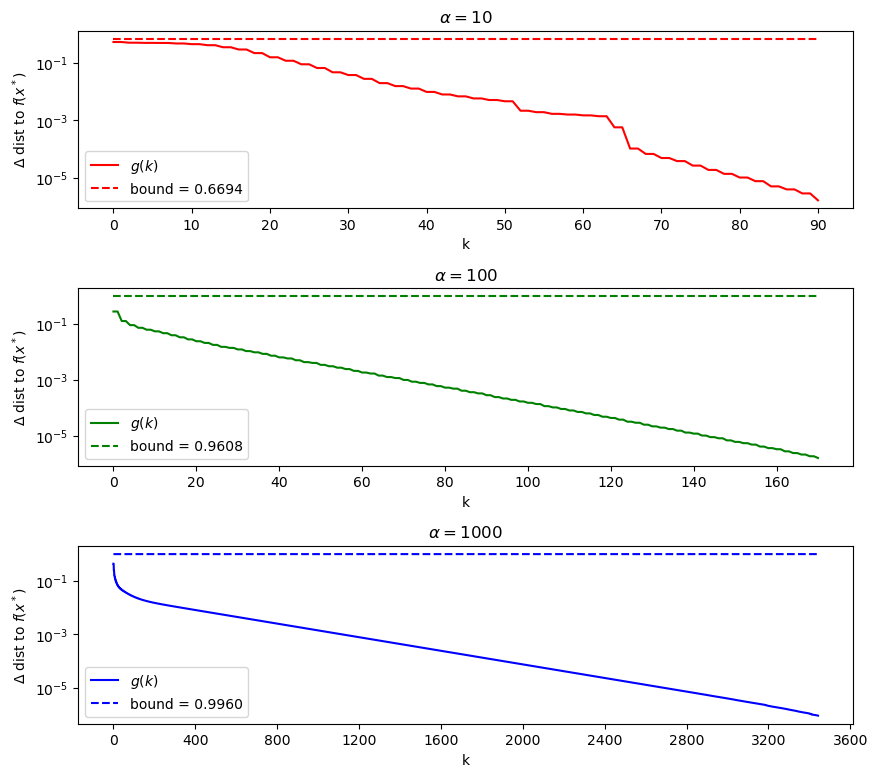
\includegraphics[width=0.7\textwidth]{plt_bound.png}
    \caption{Plot of $g(k)$ and bound 3.29 for the Ellipsoid function with $d=5$ and $\kappa(Q) = \alpha \in \{10, 100, 1000\}$}
  \label{plt3}
\end{figure}


\section{Conclusion}
I have implemented the steepest descent and Newton's method minimizers using the
backtracking line search (Algorithm 3.1) to find the step size.
The convergence plots, that I have provided, demonstrate that
the Newton's method outperforms steepest descent for all case functions,
and there is an asymptotic difference between the convergence rates of the
Steepest Descent and Newton's method, former being linear and latter being quadratic,
which agrees with the theorems in the book.
The gradient descent particularly struggles with the first three functions.
However, both methods manage to find the optima of all functions.

\end{document}


%% \section{Convergence Plots}
%% \label{sec:conv}
%% \begin{figure}[H]
%%   \centering
%%   \begin{subfigure}[b]{\textwidth}
%%     \centering
%%     \includegraphics[width=\textwidth]{plt_f_1.png}
%%     \caption{Ellipsoid Function}
%%   \end{subfigure}
%%   \begin{subfigure}[b]{\textwidth}
%%     \centering
%%     \includegraphics[width=\textwidth]{plt_f_2.png}
%%     \caption{Rosenbrock Function}
%%   \end{subfigure}
%%   \caption{Convergence Plots}
%%   \label{plt1}
%% \end{figure}
%% \end{document}
